%%% License: Creative Commons Attribution Share Alike 4.0 (see https://creativecommons.org/licenses/by-sa/4.0/)
%%% Slides are based heavily on earlier versions of this course taught by Jesper Rudiger.

\documentclass[english,10pt
%,handout
,aspectratio=169
]{beamer}
%%% License: Creative Commons Attribution Share Alike 4.0 (see https://creativecommons.org/licenses/by-sa/4.0/)
%%% Slides are based heavily on earlier versions of this course taught by Jesper Rudiger and Peter Norman Sorensen.

\DeclareGraphicsExtensions{.eps, .pdf,.png,.jpg,.mps,}
\usetheme{reMedian}
\usepackage{parskip}
\makeatother

\renewcommand{\baselinestretch}{1.1} 

\usepackage{amsmath, amssymb, amsfonts, amsthm}
\usepackage{enumerate}
\usepackage{hyperref}
\usepackage{url}
\usepackage{bbm}
\usepackage{color}

\usepackage{tikz}
\usepackage{tikzscale}
\newcommand*\circled[1]{\tikz[baseline=(char.base)]{
		\node[shape=circle,draw, inner sep=-20pt] (char) {#1};}}
\usetikzlibrary{automata,positioning}
\usetikzlibrary{decorations.pathreplacing}
\usepackage{pgfplots}
\usepgfplotslibrary{fillbetween}
\usepackage{graphicx}

\usepackage{setspace}
%\thinmuskip=1mu
%\medmuskip=1mu 
%\thickmuskip=1mu 


\usecolortheme{default}
\usepackage{verbatim}
\usepackage[normalem]{ulem}

\usepackage{apptools}
\AtAppendix{
	\setbeamertemplate{frame numbering}[none]
}
\usepackage{natbib}



\title{Financial Markets Microstructure \\ Lecture 20}

\subtitle{Asset Price Bubbles}

\author{Egor Starkov}

\date{K{\o}benhavns Unversitet \\
	Spring 2023}


\begin{document}
	\AtBeginSection[]{
		\frame<beamer>{
			\frametitle{This lecture:}
			\tableofcontents[currentsection,currentsubsection]
	}}
	\frame[plain]{\titlepage}



\begin{frame}{Previously on FMM}
	\begin{itemize}
		%\item Wrapped up \textbf{HFT}
		\item Information and trading volumes:
		\begin{itemize}
			\item Private signals create disagreement $\to$ generate trade, which reveals and aggregates private info
			\item Public signals should theoretically mitigate disagreement and lead to less trade
			\item But IRL trading volumes increase around public announcements
			\item \textbf{Kondor}: Possible explanation through second-order beliefs
		\end{itemize}
	\end{itemize}
\end{frame}	


\begin{frame}{Today}
	Two stories for why \structure{bubbles} may occur
	\begin{itemize}
		\item Rational herding
		\begin{itemize}
			\item Herding: following the actions of others, even when this goes against one's own private information
			\item We will look at different explanations for why this may be rational
		\end{itemize}
		\item Lack of common knowledge/coordination (\cite{abreu_bubbles_2003})
		\begin{itemize}
			\item There is a difference between everybody knowing that an asset is overpriced, and everybody knowing that everybody knows...
			\item Again, speculation depends on these \emph{higher-order beliefs}
		\end{itemize}
	\end{itemize}
\end{frame}


\begin{frame}{Bubbles}
	\begin{itemize}
		\item \textbf{Wikipedia}: ``Trade in high volumes at prices that are considerably at variance with intrinsic values''
		\item \textbf{Investopedia}: ``A surge in equity prices, often more than warranted by the fundamentals and usually in a particular sector, followed by a drastic drop in prices as a massive sell-off occurs''
		\item \textbf{Chicago Fed}: ``...a bubble exists when the market price of an asset exceeds its price determined by fundamental factors by a significant amount for a prolonged period''
	\end{itemize}
	%Here are some \hyperlink{examples}{\beamerbutton{examples}}
\end{frame}


%\begin{frame}{Examples of bubbles}
%	\begin{columns}
%		\begin{column}{0.45\linewidth}
%			\center
%			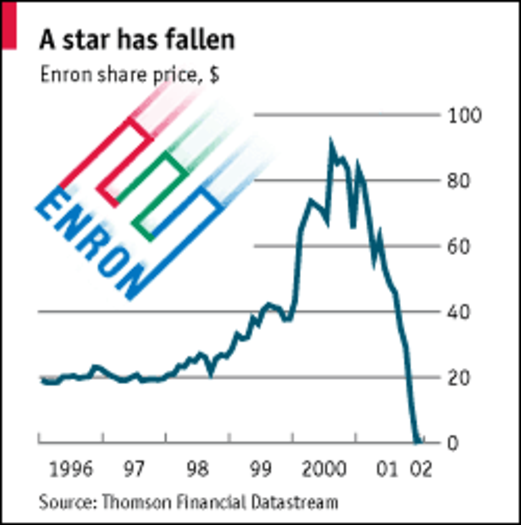
\includegraphics[width=0.95\linewidth]{pics/Enron}
%		\end{column}
%		\begin{column}{0.55\linewidth}
%			\begin{itemize}
%				\item \textbf{Enron} was an energy company that grew spectacularly throughout the nineties; named America's most innovative company
%				\item But in October 2001 it was revealed that the company had hid billions of dollars of debts; stock price plummeted
%				\item Looks like a bubble -- but could market have done better?
%			\end{itemize}
%		\end{column}
%	\end{columns}
%\end{frame}


\begin{frame}[handout:0]{Examples of bubbles}
	\begin{columns}
		\begin{column}{0.55\linewidth}
			\center
			\only<1>{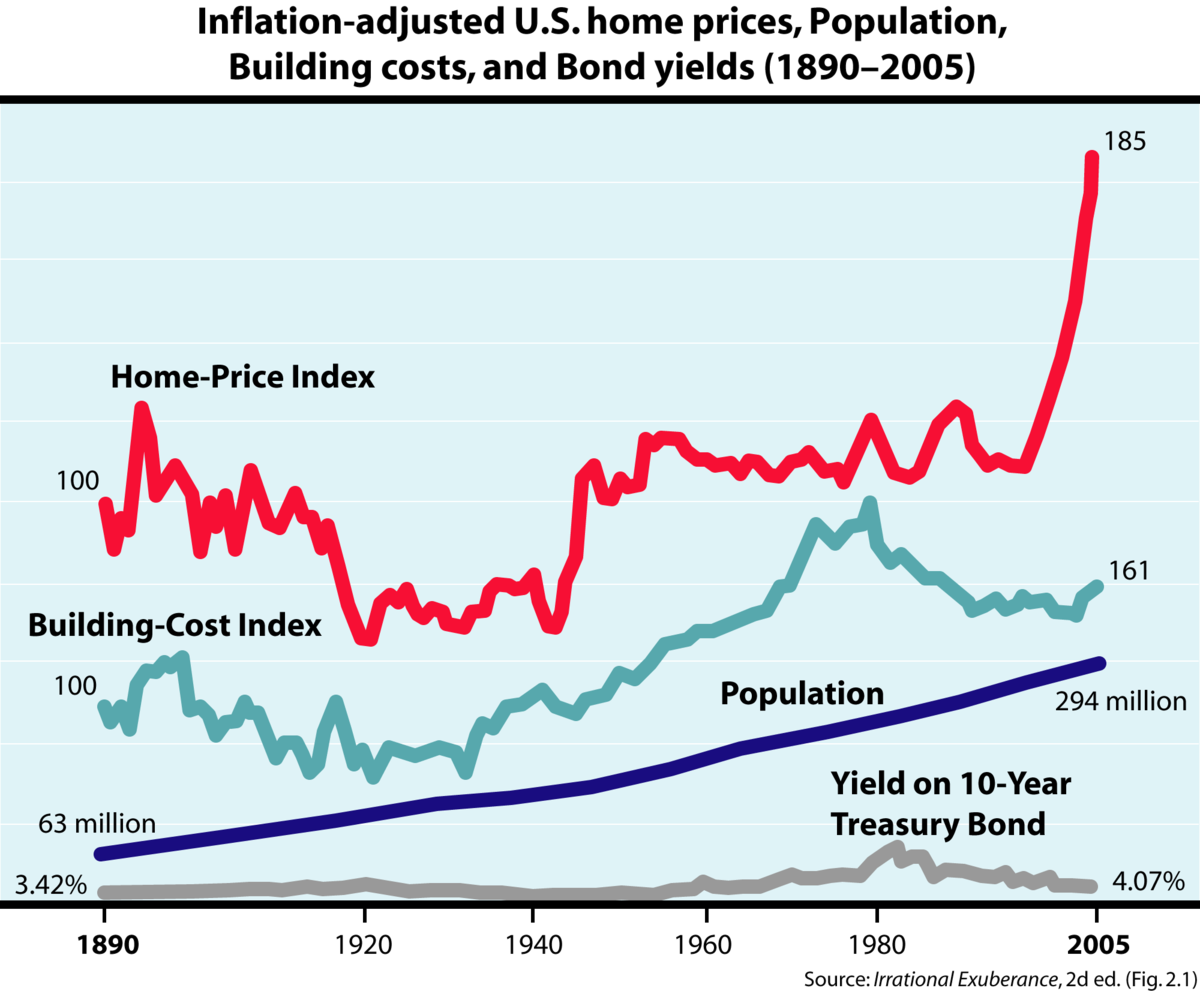
\includegraphics[width=0.95\linewidth]{pics/housing}}
			\only<2>{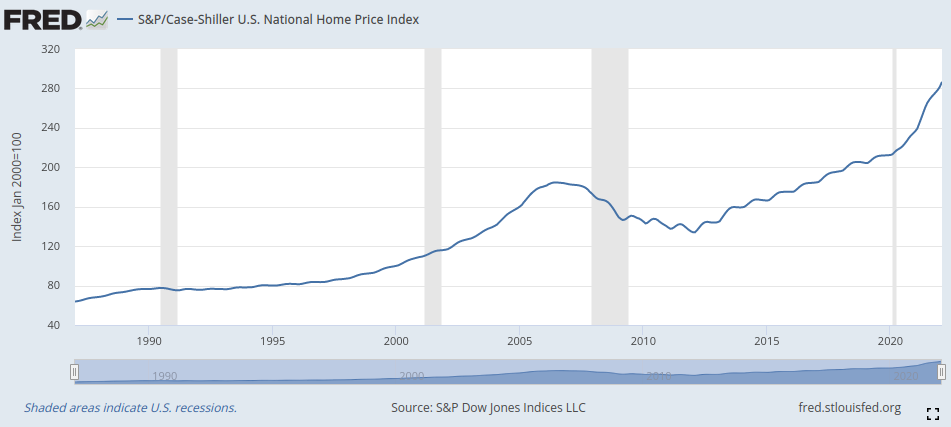
\includegraphics[width=0.95\linewidth]{pics/housing2}}
		\end{column}
		\begin{column}{0.45\linewidth}
			\begin{itemize}
				\item US \textbf{housing} market had a bubble in mid-2000s
				\item Its burst was a significant contributor to the Great Recession
			\end{itemize}
		\end{column}
	\end{columns}
\end{frame}


\begin{frame}[handout:0]{Examples of bubbles}
	\begin{columns}
		\begin{column}{0.55\linewidth}
			\center
			\only<1>{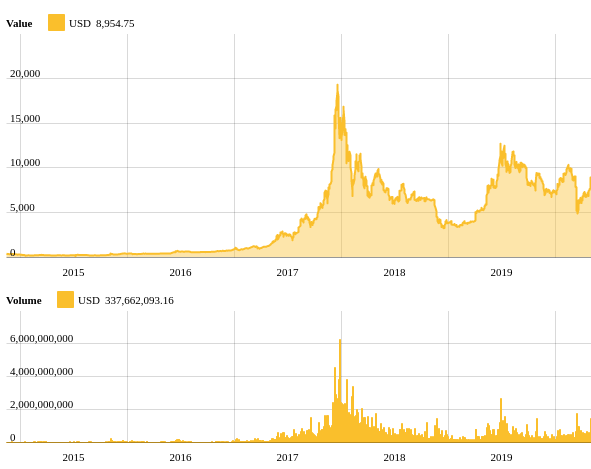
\includegraphics[width=\linewidth]{pics/bitcoin}}
			\only<2>{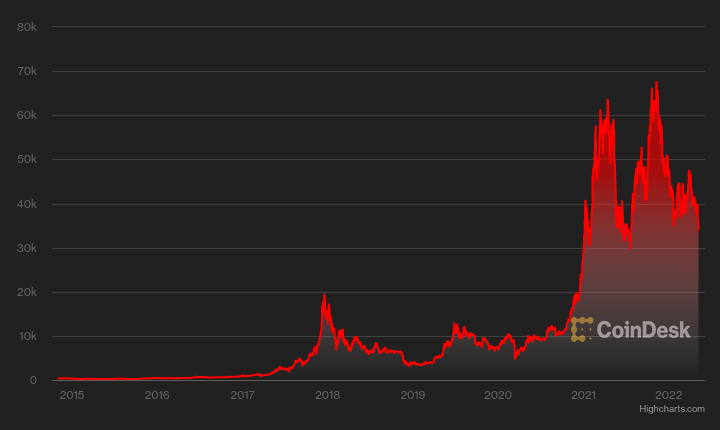
\includegraphics[width=\linewidth]{pics/bitcoin2}}
		\end{column}
		\begin{column}{0.45\linewidth}
			\begin{itemize}
				\item \textbf{Bitcoin} grew and burst pretty badly at the end of 2017.
				\pause 
				\item ...and is just pretty volatile overall
				\item (to be fair, like with any fiat currency, not clear what bitcoin's fundamental value is, so can say that any positive price is a bubble)
			\end{itemize}
		\end{column}
	\end{columns}
\end{frame}


\begin{frame}[handout:0]{Examples of bubbles}
\begin{columns}
	\begin{column}{0.7\linewidth}
		\center
		\includegraphics[width=\linewidth]{pics/gme}
	\end{column}
	\begin{column}{0.3\linewidth}
		\begin{itemize}
			\item we remember the \textbf{Gamestop} frenzy of January 2021...
		\end{itemize}
	\end{column}
\end{columns}
\end{frame}


\begin{frame}[handout:0]{Examples of bubbles}
	\begin{columns}
		\begin{column}{0.55\linewidth}
			\center
			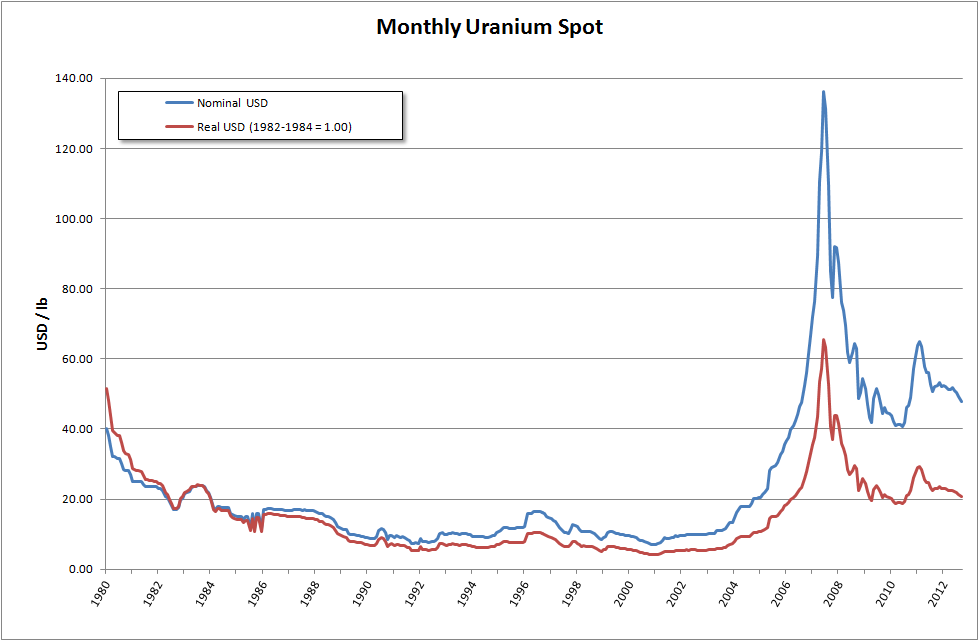
\includegraphics[width=\linewidth]{pics/Uranium}
		\end{column}
		\begin{column}{0.45\linewidth}
			\begin{itemize}
				\item In the early noughties, the price of \textbf{uranium} was upward trending
				\item In late 2006 the Cigar Lake Mine in Canada containing the largest known undeveloped reserves was flooded
				\item This seemingly set off an uncontrolled increase in price followed by a crash: classic bubble behavior
			\end{itemize}
		\end{column}
	\end{columns}
\end{frame}






\section{Herd Behavior in Financial Markets}

\begin{frame}{Herding: Introduction}
	\begin{itemize}
		\item \textbf{Herding}: ignoring private information in favor of ``wisdom of the crowd''
		\begin{enumerate}
			\item Herding may be the efficient response to new information or similarity between agents...
			\item ...but it may also be the inefficient result of a certain decision making process. Here: focus on the latter
		\end{enumerate}
		\item In \textbf{financial markets}: momentum trading, positive-feedback trading
		\item In 1992, a wave (a herd?) of articles showing that  herding could be result of rational \structure{informational cascade}
		\item Today we look at this and other `rational' explanations
		\item Note: I will follow the presentation in \cite{bikhchandani_herd_2000}. 
		\\See \cite{bikhchandani_information_2021} for a comprehensive review of the literature.
	\end{itemize}
\end{frame}


\begin{frame}{Preview}
	\begin{itemize}
		\item Agents arrive at the market sequentially and need to make a decision
		\item Every agent has a private signal and observes decisions of previous agents (but not their signals!)
		\item Ideally: pool private information to find best decision
		\item But here: \structure{sequential decision making}
		\begin{itemize}
			\item First-comers: make decisions based on information
			\item But as time goes by, people may start disregarding their own
			\\ information and just choose the most popular action
			\item Herding ensues, but it is \emph{fully rational}: public information swamps private information
		\end{itemize}
		\item \structure{Informational cascade}: a few pieces of information may determine everyone's choice
	\end{itemize}
\end{frame}


\begin{frame}{Model}
	\begin{itemize}
		\item \textbf{State} (fundamental) $v \in \{L,H\}$;
		\item In each period $t \in \{1,2, ...\}$ an individual arrives and needs to make a \textbf{decision} $d_t \in \{0,1\}$ (invest or not);
		\item \textbf{Payoffs} $u(d_t,v)$:
		\begin{itemize}
			\item $u(0,v) = 0$,
			\item $u(1,L) = L-m < 0$,
			\item $u(1,H) = H-m > 0$,
			\item (say for now that price (midquote) $m$ is fixed and there is no spread: $a=b=m$)
		\end{itemize}
	\end{itemize}
\end{frame}


\begin{frame}{Model: Beliefs}
	\begin{itemize}
		\item Represent all beliefs $p$ about $v$ as probabilities of $v=H$ conditional on relevant info.
		\item \structure{``Market belief''} $q_t$
		\begin{itemize}
			\item $q_0$ is the public prior belief -- e.g., $1/2$;
			\item $q_t$ incorporates info contained in decisions at $t = 1,2,...,t-1$
		\end{itemize}
		\item Period-$t$ agent observes $q_t$ and a \structure{private signal} $\eta_t$ and forms \structure{private belief} $r_t$.
		\begin{itemize}
			\item Suppose $\eta_t \in \{h,l\}$ with $\mathbb{P}(\eta_t=h | v=H) = \mathbb{P}(\eta_t=l | v=L) = \rho$.
		\end{itemize}
		\item All beliefs calculated using Bayes' rule
	\end{itemize}
\end{frame}


\begin{frame}{Decisions}
	\begin{itemize}
		\item Agent behaves optimally $\Rightarrow$ chooses $d_t=1$ iff $r_t \geq \bar{r} \equiv \frac{m-L}{H-L}$.
		\item Use Bayes' rule to compute $r_t(\eta_t,q_t)$:
		%\[r_t = \frac{p_t q_t}{p_t q_t + (1-p_t) (1-q_t)}\]
		\begin{align*}
			r_t(h,q_t) &= \frac{q_t \rho}{q_t \rho + (1-q_t) (1-\rho)}
			\\
			r_t(l,q_t) &= \frac{q_t (1-\rho)}{q_t (1-\rho) + (1-q_t) \rho}
		\end{align*}
		Note $r_t(h,q_t) > q_t > r_t(l,q_t)$.
	\end{itemize}
\end{frame}


\begin{frame}{Herds and cascades}
	\begin{itemize}
		\item If $r_t(h,q_t) > \bar{r} > r_t(l,q_t)$ then the agent follows their signal 
		\\$\to$ their action is informative 
		\\$\to$ public belief is updated: $q_{t+1}(q_t,d_t=1) = r_t(h,q_t)$; $q_{t+1}(q_t,d_t=0) = r_t(l,q_t)$.
		
		\item If $r_t(h,q_t) > r_t(l,q_t) > \bar{r}$ then the agent chooses $d_t=1$ regardless of private signal 
		\\$\to$ action uninformative $\to$ $q_{t+1} = q_t$ 
		\\$\to$ next agent will also ignore private signal!
		\begin{itemize}
			\item Everyone ignores private signals and chooses the same action (we have a \alert{herd})
			\item Market belief $q_t$ is frozen in place; private information is not aggregated!
			\item This \alert{herd may be incorrect} (unless $q_t=0$ or $q_t=1$)
			\item (Same happens if $\bar{r} > r_t(h,q_t) > r_t(l,q_t)$ with $d_t=0$)
		\end{itemize}
	\end{itemize}
\end{frame}


\begin{frame}{What triggers the herd?} \label{HERD}
	\begin{itemize}
		\item A few incorrect signals can be enough enough to set off a herd
		\item A small piece of information `cascades' through the system
		\item Each agent is rational, but together they may seem stupid: their information taken together is very precise, but there is no information aggregation
		\item A specific example with numbers of how a herd may arise: \hyperlink{EXP}{\beamerbutton{here}}
	\end{itemize}
\end{frame}


\begin{frame}{Herds and cascades: comments}
	\begin{itemize}
		\item Incorrect herds only occur if distribution of $\eta_i$ is bounded -- otherwise strong enough signals could overpower the public info
		\item In a slightly richer model, the opposite outcome is also possible -- state of permanent uncertainty in which everyone acts solely on their private signal, ignoring public information
		\item Terminology:
		\begin{itemize}
			\item \structure{Herd} = action convergence ($d_{t+1} = d_t$ from some point onwards)
			\item \structure{Cascade} = public belief convergence ($q_{t+1} = q_t$ from some point onwards)
			\item Distinction is not super important for our purposes
		\end{itemize}
	\end{itemize}
\end{frame}


\begin{frame}{What if we introduce a price?}
	\begin{itemize}
		\item As before: unknown asset value $v$, and each trader receives a private signal $\eta_i$
		\item With probability $\pi$ the trader is a noise trader, who buys/sells/abstains with equal probability, w.p. $1-\pi$ rational as above
		\item A risk-neutral market maker quotes competitive bid-ask \structure<1>{prices}
		\item What will happen?
		\begin{itemize}
			\pause
			\item This is standard Glosten-Milgrom, so no herds!
			\item Prices adjust in such a way that following private signals is optimal, and prices themselves then incorporate all private signals!
		\end{itemize}
	\end{itemize}
\end{frame}


\begin{frame}{More layered model}
	\begin{itemize}
		\item However, the GM result is in part due to model simplicity
		\item \cite{avery_multidimensional_1998} expand on this analysis
		\begin{itemize}
			\item Suppose $v \in \{0,\frac{1}{2},1\}$
			\item If $v=\frac{1}{2}$, this is perfectly revealed by the private signal: $\eta_{t}=\frac{1}{2}$
			\item If $v \in \{0,1\}$, trader $t$ receives informative signal with precision $\rho_t \equiv \mathbb{P}(\eta_{t}=v)$
			\item Furthermore, a proportion $\mu \in \{\mu^{H}, \mu^{L}\}$ of traders have perfect information: $\rho_{t}=1$ after a good signal
			\item The remaining traders have noisy info: $\rho_{t} \in (\frac{1}{2},1)$ after a good signal
		\end{itemize}
		\pause
		\item Three levels of uncertainty (for MM): 
		\begin{itemize}
			\item Event uncertainty: $v=1/2$ (\alert{no event}) or $v \in \{0,1\}$ (\structure{event})
			\item Value uncertainty: if event, \structure{$v=1$} or \alert{$v=0$}
			\item Composition uncertainty: many informed traders ($\mu^{H}$: \structure{well-informed economy}) or few ($\mu^{L}$: \alert{poorly-informed economy})
		\end{itemize}
	\end{itemize}
\end{frame}


\begin{frame}[label=az]
	\frametitle{Herding can occur with pricing and multi-layered uncertainty}
	\begin{itemize}
		\item In GM, price mechanism worked as a screening device: made sure that high types bought and low types sold
		\item But now, it is possible to `misprice' such that herding occurs, at least temporarily
		\begin{itemize}
			\item Can be because $\mu = \mu_H$ so all traders know $v$, but MM does not (non-speculative bubble)
			\item Can be because $\mu = \mu_L$ but traders do not know that and perceive past order flow as more informative than it is (speculative bubble)
		\end{itemize}
		\item This allows bubbles to occur
	\end{itemize}
	See numerical example \hyperlink{layers}{\beamerbutton{here}}
\end{frame}


\begin{frame}{Other types of herding: Reputational herding}
	A brief example.
	\begin{itemize}
		\item \textbf{Two  managers}: Invest or not in project of unknown value (gets imperfect signal $\eta \in \{1,0\}$)
		\item \textbf{Type}: Each manager either smart or dumb (doesn't know). If both managers smart, observe same $\eta$; if one or both dumb, observe independent signals $\eta$ %(also uncorrelated with $v$)
		\item \textbf{Payoffs}:  Managers \structure{maximizes their reputation} (want to appear smart)
		\item \textbf{Herding}: Manager 1 moves first, then manager 2 
		\begin{itemize}
			\item If manager 1 invests, manager 2 can deduce that $\eta_1=1$. Suppose $\eta_2=0$. 
			\\ Then one of the two (or both) must be dumb. 
			\item If manager 2 does not invest, he reveals this. If player 1's investment then 
			\\succeeds, people will assume that manager 2 is the dumb manager
			\item Investing might be better: even if the investment fails, people might think that 
			\\both managers are smart, but got an `unlucky' signal
		\end{itemize}
	\end{itemize}
\end{frame}


\begin{frame}{Herding: Conclusion}
	\begin{itemize}
		\item \textbf{Herding}: may occur when private information cannot be easily aggregated
		\item \textbf{Price mechanism}: alleviates problem by providing private incentives to trade and thus reveal information, which is then incorporated into prices
		\item \textbf{Multi-layered uncertainty}: can make the herds occur even with flexible prices
		\item \textbf{Aside}: \emph{Momentum trading} often assumed to be a `behavioral feature': but it may be perfectly rational
		\item \textbf{Empirical estimation of herding}: some conclusions can be tested in the data but to a very limited extent; see \cite{bikhchandani_herd_2000} and \cite{bikhchandani_information_2021} for details.
	\end{itemize}
\end{frame}




\section{Abreu and Brunnermeier: Bubbles and Crashes}

\begin{frame}{\cite{abreu_bubbles_2003}: Introduction}
	\begin{itemize}
		\item Efficient market hypothesis: bubbles are impossible
		\begin{itemize}
			\item In finite model, use backward induction argument: no mispricing in last period, which should be foreseen in second-last period, etc. $\rightarrow$ unravelling
		\end{itemize}
		\item This requires that all traders agree on when the bubble will collapse (at least on the distribution of times)
		\item Here: a model in which coordination is needed to cause a crash
		\item Coordination, in turn, depends on beliefs about others
		\begin{itemize}
			\item Back to higher order beliefs
		\end{itemize}
	\end{itemize}
\end{frame}


\begin{frame}{Model}
	\begin{itemize}
		\item \textbf{Single asset traded}: value at $t$ is $v_t$
		\item \textbf{Progress}: At $t=0$, technological progress  makes $v_t$ grow at rate $g$
		\item \textbf{Slowdown}: at some random time $t_0$, there is a slowdown and $v_t$ growth slows to $r<g$
		\item \textbf{Price}: Price grows at rate $g$ until either
		\begin{itemize}
			\item At least a fraction $\kappa$ of rational traders sell the asset ($\kappa$ is the \emph{absorption capacity} of the economy), or
			\item The market is exogenously corrected at time $t_0+\overline{\tau}$
		\end{itemize}
		\item \textbf{Gradual learning}: Each period, a fraction $1/\eta$ of rational traders 
		\\become aware of the mispricing
		\begin{itemize}
			\item But they don't know $t_0$, and hence don't know 
			\\how many others know of the mispricing
		\end{itemize}
	\end{itemize}
\end{frame}


\begin{frame}{Traders}
	\begin{itemize}
		\item \textbf{Behavioral traders} think progress will last forever
		\begin{itemize}
			\item When enough rational traders sell, absorption capacity of behavioral traders is reached and  price must drop
			\item At this point, everybody becomes aware of the mispricing
			\item If this doesn't happen, then market exogenously collapses when mispricing is too big
		\end{itemize}
		\item \textbf{Rational traders} know progress is temporary, but not when it stops
		\begin{itemize}
			\item Implication: when you learned that progress has stopped, you are not sure what other people believe
			\item Suppose you learn at $t'$. At $t' + \eta$ you know that everybody knows
			\item But somebody else might learn that progress stopped at $t''>t'$; he will not know that everybody knows until $t''+\eta>t'+\eta$
		\end{itemize}
	\end{itemize}
\end{frame}


\begin{frame}{Graphically}
	\center
	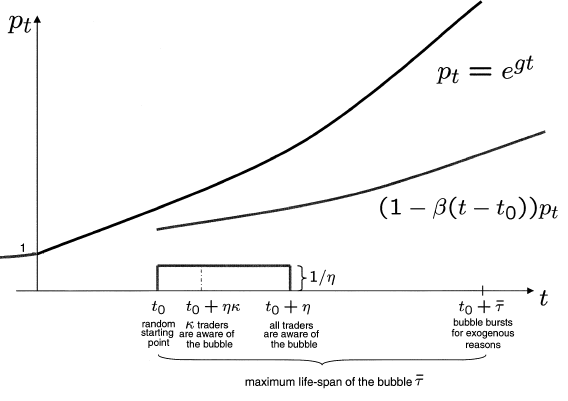
\includegraphics[width=0.57 \paperwidth]{pics/AbreuBrun}
	
	(Note: graph is from the paper and it has a mistake)
\end{frame}


\begin{frame}{Why bubbles then?}
	\begin{itemize}
		\item In this model there is never \emph{common knowledge}: you are never sure what the others know. This prevents usual backward induction
		\item At least $\kappa$ traders must sell to burst bubble: coordination important
		\item But it is hard to coordinate without common knowledge
		\item Therefore, mispricing can go on for a long time
		\begin{block}{}
			Even if traders realize the market will crash, they don't know exactly when, incentivizing them to ride the bubble
		\end{block}
	\end{itemize}
\end{frame}


\begin{frame}{Definition of a bubble}
	\begin{itemize}
		\item In this setting, let's use a very strict definition of a bubble
		\item In particular, notice that after $t_0+\eta\kappa$, the mispricing is known by enough traders to correct it
		\begin{block}{Definition}
			A bubble is persistent mispricing \emph{beyond $t_0+\eta \kappa$}
		\end{block}
		\item Thus, in this definition it is not enough that the asset is priced over its value for there to be a bubble
		\item The mispricing must be well-known to traders
	\end{itemize}
\end{frame}


\begin{frame}{Some observations}
	The following is shown in the paper:
	\begin{itemize}
		\item Traders either take the maximum long (buy) or short (sell) position
		\item When a rational trader `goes short', all traders who learned of the mispricing before him will already have gone short
		\item Once a rational trader goes short, he never re-enters the market: he waits for the bubble to burst
	\end{itemize}
\end{frame}


\begin{frame}{Bubbles and crashes}
	Generally, in the model, there are two possible types of equilibria
	\begin{itemize}
		\item Exogenous crash
		\begin{itemize}
			\item When the growth rate $g$ under the bubble is high, dispersion $\eta$ and absorption capacity $\kappa$ are high,  informed traders sell out very slowly
			\item In effect, they take a chance on `riding the bubble'
			\item As a result, selling will never be sufficient to burst the bubble, which will burst at the exogenous date $t_0+\overline{\tau}$
		\end{itemize}
		\item Endogenous crash
		\begin{itemize}
			\item When traders have incentives to sell quick, this leads to unraveling: enough traders will sell to make the bubble burst
			\item However, `bubble incentives' remain: the sooner the price crashes, the smaller the cost of riding the bubble
			\item Therefore, the bubble will be smaller but still exist
		\end{itemize}
	\end{itemize}
\end{frame}


\begin{frame}{The role of `sunspots'}
	\begin{itemize}
		\item \textbf{Sunspot equilibria}: refers to equilibria where \emph{economically irrelevant information} has an influence
		\item In our case: suppose an uninformative event is observed with a certain probability 
		\item If informed traders decide to coordinate their actions around this event (eg. use the strategy `sell when event occurs'), it can become pivotal
		\item Example from article: in 1980s trade data had big market impact in the US; in 1990s Alan Greenspan's statements were more influential
		\begin{itemize}
			\item If sufficiently many people react to an event you must too - even if the event carries little/no information by itself
		\end{itemize}
	\end{itemize}
\end{frame}


\begin{frame}{Abreu and Brunnermeier: Conclusion}
	\begin{itemize}
		\item Standard arguments against bubbles rely a lot on common knowledge between agents
		\item When we dispense with common knowledge, belief dispersion among agents can cause mispricings to persist even after everyone has observed the mispricing
		\item Thus, bubbles may not be fixed by the market
		\item As a side-effect, seemingly insignificant events can serve to coordinate actions and cause crashes
	\end{itemize}
\end{frame}


%\begin{frame}{Next time: auctions}
%	\begin{itemize}
%		\item Look at models of how traders bid for the asset under imperfect competition from other bidders
%		\item Extracurricular
%	\end{itemize}
%\end{frame}




\appendix
\begin{frame}<handout:0>[allowframebreaks]{References}
	\bibliography{../teaching}
	\bibliographystyle{abbrvnat}
\end{frame}


\begin{frame}{Herding example: Setup} \label{EXP}
	\begin{itemize}
		\item This example follows that in \cite{bikhchandani_herd_2000}
		\item Suppose $q_0 = 1/2$
		\item \textbf{Payoffs}: Let $L-m = -1$; $H-m = 1$
		\begin{itemize}
			\item Then $\bar{r} = 1/2$
			\item Suppose that agents flip a $50/50$ coin whenever indifferent
		\end{itemize}
		\item Suppose the following signal sequence realized: $\{\structure{h},\alert{ l, l, l, ...}\}$
		\item Denote by $\mathbb{I}_i$ agent $i$'s information set
	\end{itemize}
\end{frame}


\begin{frame}{Herding example: Analysis}
	\textbf{First agent}
	\begin{itemize}
		\item Information set $\mathbb{I}_1=\{\eta_1=h\}$
		\item Then
		\[
			r_1(h,1/2) = \mathbb{P}(v=H|\mathbb{I}_1) = \frac{\frac{1}{2} \rho}{\frac{1}{2} \rho+\frac{1}{2} (1- \rho)} = \rho 
		\]
		\item Since $\rho>1/2$: invest.
		\item \textbf{Thus}, given $\eta_1=h$, first agent invests: $d_1=1$
	\end{itemize}
\end{frame}


\begin{frame}{Herding example: Analysis (2)}
	\textbf{Second agent}
	\begin{itemize}
		\item Second agent can perfectly deduce first agent's signal: $\eta_1=h$ if $d_1=1$, $\eta_1=l$ otherwise.
		\begin{itemize}
			\item In other words, $q_2 = r_1 = \rho$, no information is lost.
			\item Second agent receives $\eta_2=l$, his information set is $\mathbb{I}_2=\{\eta_1=1,\eta_2=-1\}$
		\end{itemize}
		\item Signals are \emph{symmetric}, so
		\[ r_2(l,\rho) = \mathbb{P}(v=H|\mathbb{I}_2) = \frac{\frac{1}{2} \rho(1-\rho)}{\frac{1}{2} \rho(1-\rho)+\frac{1}{2} (1-\rho)\rho} = 1/2 \]
		\item Thus, second agent is indifferent, flips a coin to decide. If $d_2 = 0$ then we are back to $q_3=1/2$.
		\item But suppose the coin-toss decides invest: $d_2=1$
	\end{itemize}
\end{frame}


\begin{frame}{Herding example: Analysis (3)}
	\textbf{Third agent}
	\begin{itemize}
		\item Third agent can also perfectly deduce the first agent's signal
		\item Information set is $\mathbb{I}_3=\{\eta_1=h, d_2=1, \eta_3=l\}$. Furthermore,  
		\begin{align*}
		\mathbb{P}(d_2=1|v=H)	&= \rho +(1-\rho) (1/2)=(1+\rho)/2\\
		\mathbb{P}(d_2=1|v=L)	&= \rho(1/2) +(1-\rho)=1-\rho/2
		\\
		\Rightarrow q_3(q_2=\rho,d_2=1) &= \frac{\rho \frac{1+\rho}{2}}{\rho \frac{1+\rho}{2} + (1-\rho) \left(1-\frac{\rho}{2}\right)}
		\\
		\Rightarrow r_3(l,q_3) &= 
		 \frac{\rho \frac{1+\rho}{2}(1-\rho)}{\rho\frac{1+\rho}{2}(1-\rho) + (1-\rho) \left(1-\frac{\rho}{2}\right)\rho} 
		=\frac{1+\rho}{3}>\frac{1}{2}
		\end{align*}
		\item Hence, $d_3=1$
	\end{itemize}
\end{frame}


\begin{frame}{Herding example: Analysis (4)}
	\textbf{Fourth agent}
	\begin{itemize}
		\item Information set   $\mathbb{I}_4=\{\eta_1=h,d_2=d_3=1, \eta_4=l\}$
		\item Agent four knows that agent three would have invested regardless of his signal
		\item So he doesn't learn anything from $d_3$. So $q_4 = q_3$ and $r_4(l,q_4) = r_3(l,q_3)$
		\item Hence $d_4=1$
		\item Same for all subsequent agents: $d_i=1$ for all $i$, regardless of $\eta_i$!
		\item We have a herd! -- and a very inefficient one at that! (Look at signals) \hyperlink{HERD}{\beamerbutton{back}}
	\end{itemize}
\end{frame}



\begin{frame}{Herding with prices example} \label{layers}
	Take an extreme case of Avery and Zemsky's model: suppose the following parameter values
	\begin{itemize}
		\item $\mathbb{P}(v=1/2)=0.9999$: very small prior probability of an `event'; $\mathbb{P}(v=1)=\mathbb{P}(v=0)=0.00005$
		\item $\frac{\mathbb{P}(\mu=\mu^{H})}{\mathbb{P}(\mu=\mu^{L})}=99$: high prior probability of a well-informed economy
		\item If economy is poorly informed: all traders have $p_{i}=0.51$, i.e. very poor signal about value
	\end{itemize}
	Suppose we're in an unlikely state of the world
	\begin{enumerate}
		\item Value is low ($v=0$) implying that there is an event
		\item The economy is poorly informed ($\mu=\mu^L$)
	\end{enumerate}
	How will  market learn state of the world? Let's look at a  simulation
\end{frame}


\begin{frame}{Herding with prices example (2)}
	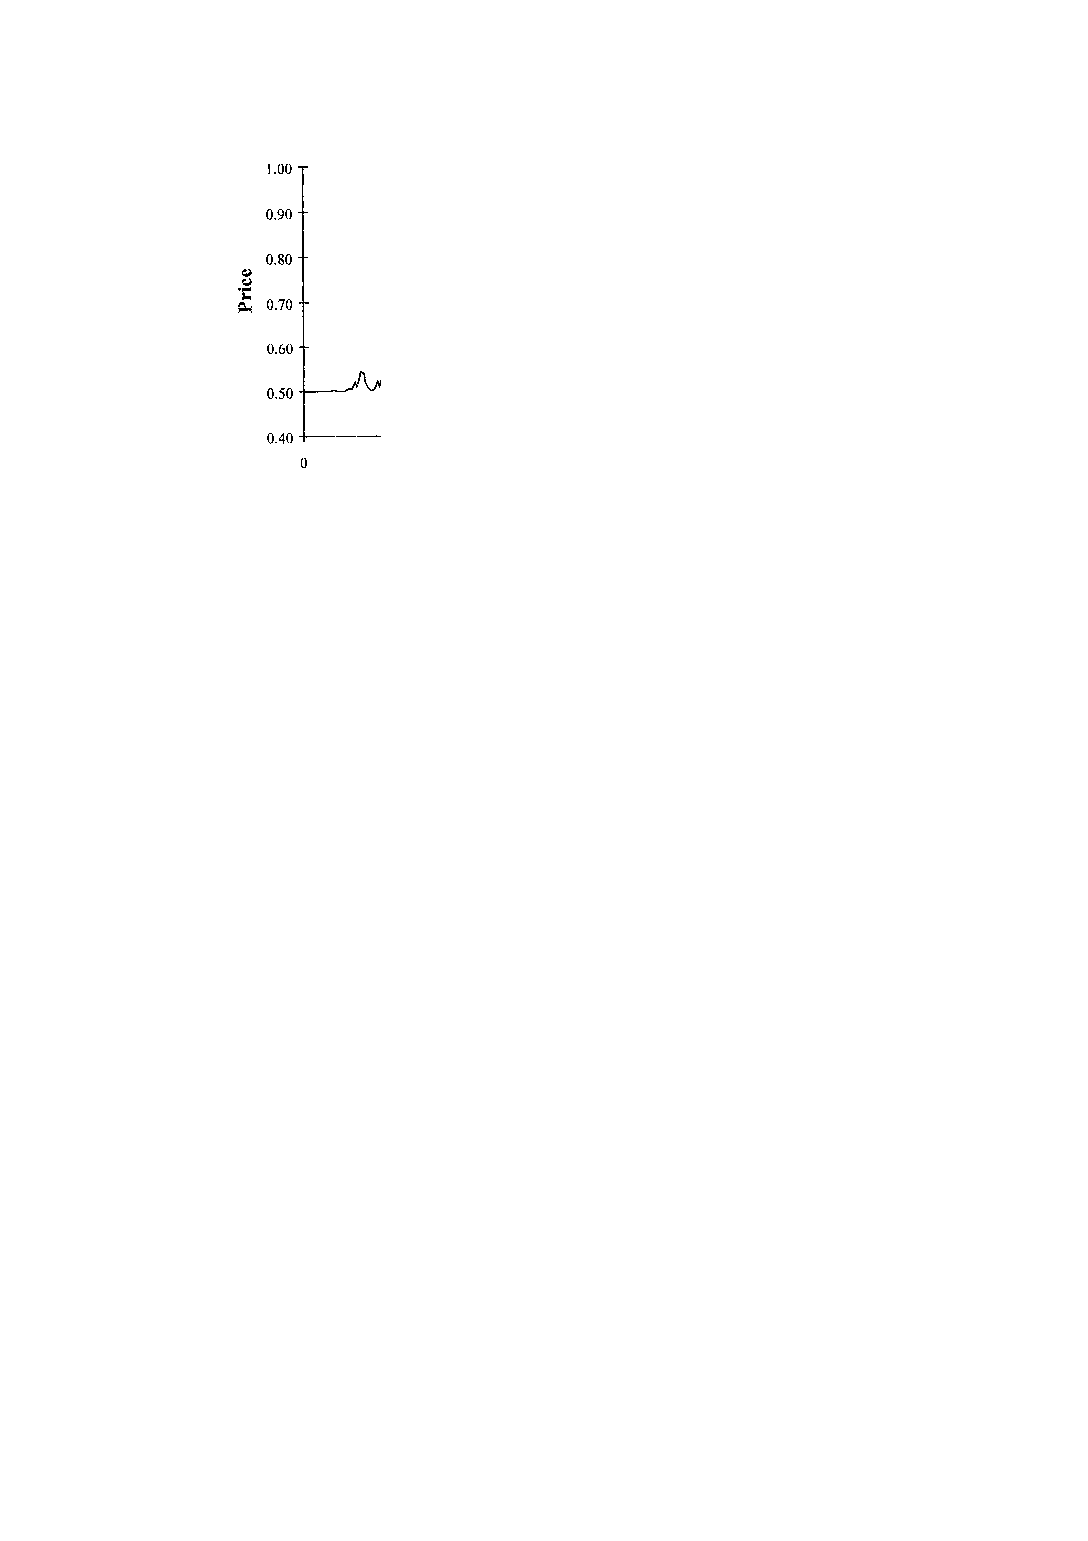
\includegraphics[width=0.10\paperwidth]{pics/PriceBubble1} \hfill
	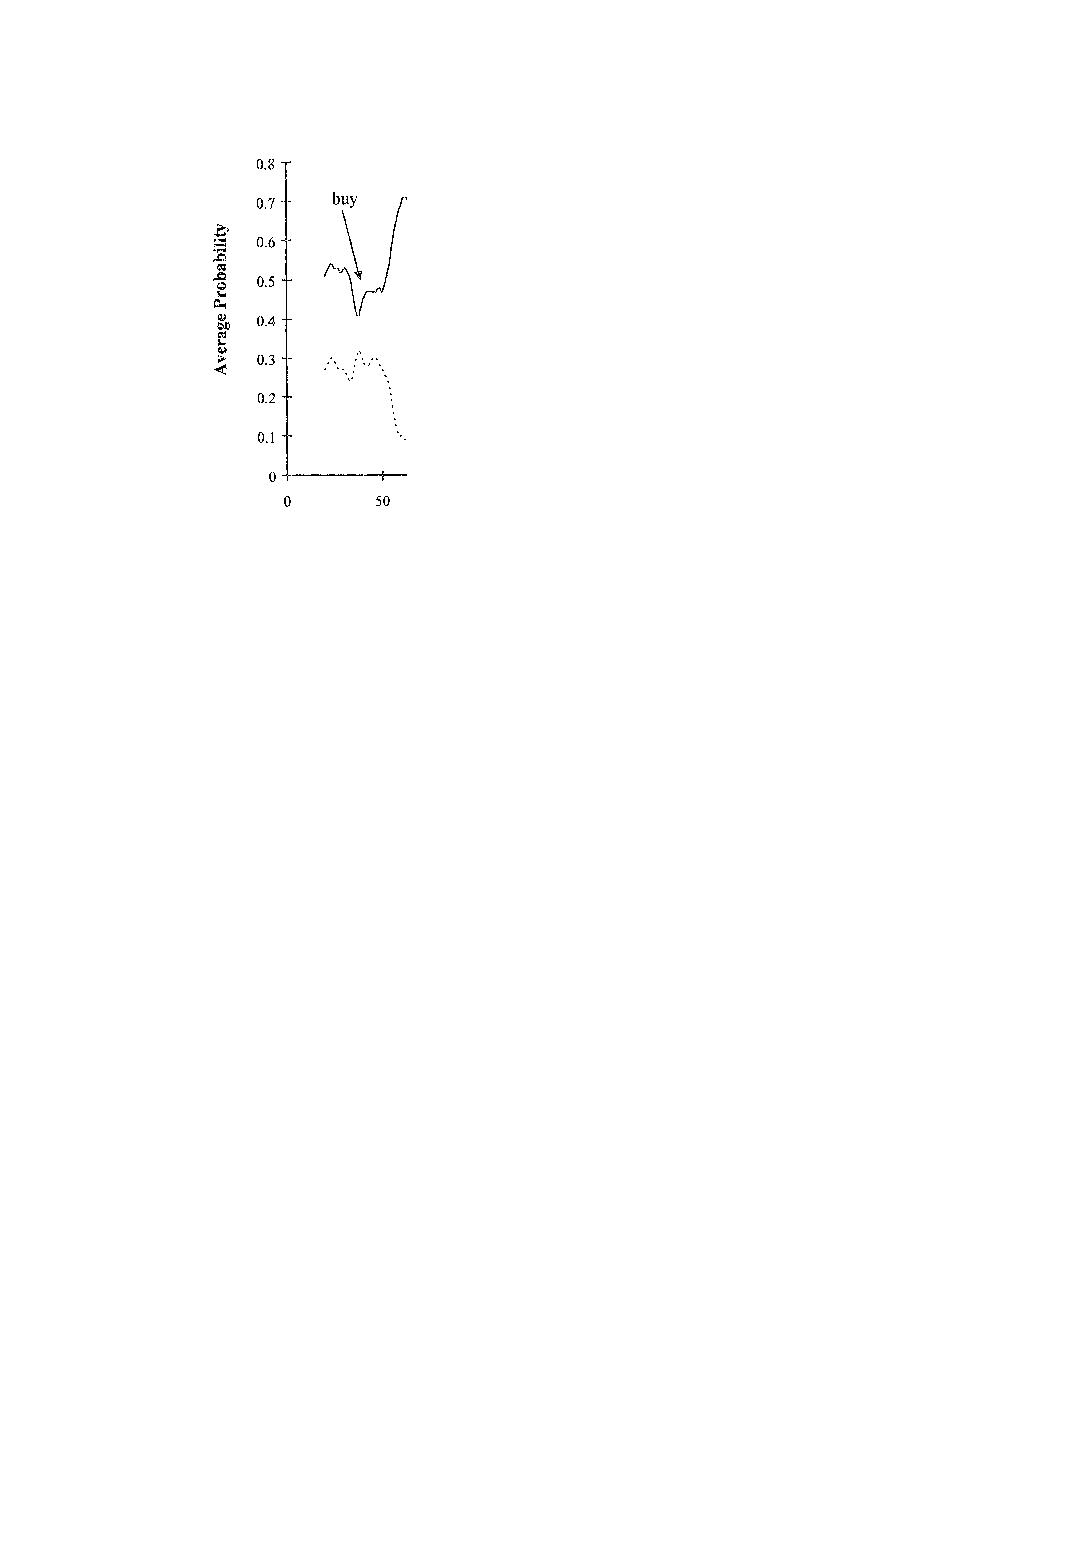
\includegraphics[width=0.12\paperwidth]{pics/Trade1} \hfill \hfill
	
	Three of first five traders buy  
	\begin{itemize}
		\item Since economy poorly informed: herd buying starts
		\item MM thinks it's likely that economy is well informed: price goes up
	\end{itemize}
\end{frame}


\begin{frame}{Herding with prices example (3)}
	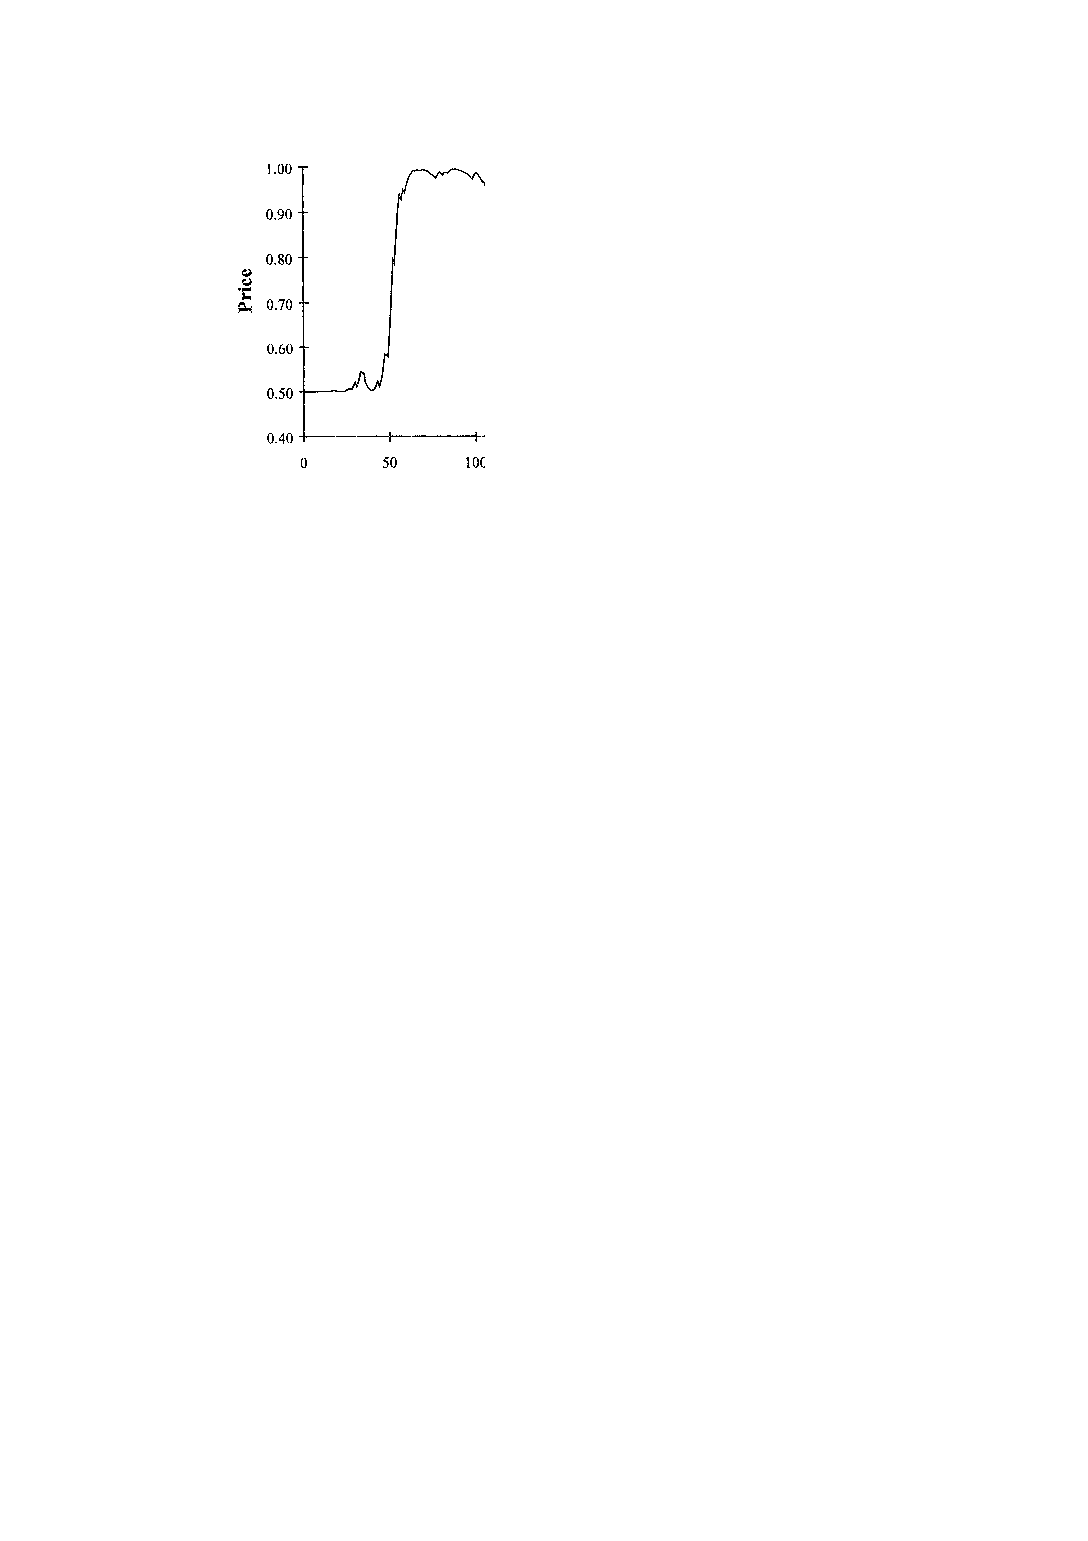
\includegraphics[width=0.17\paperwidth]{pics/Price2} \hfill
	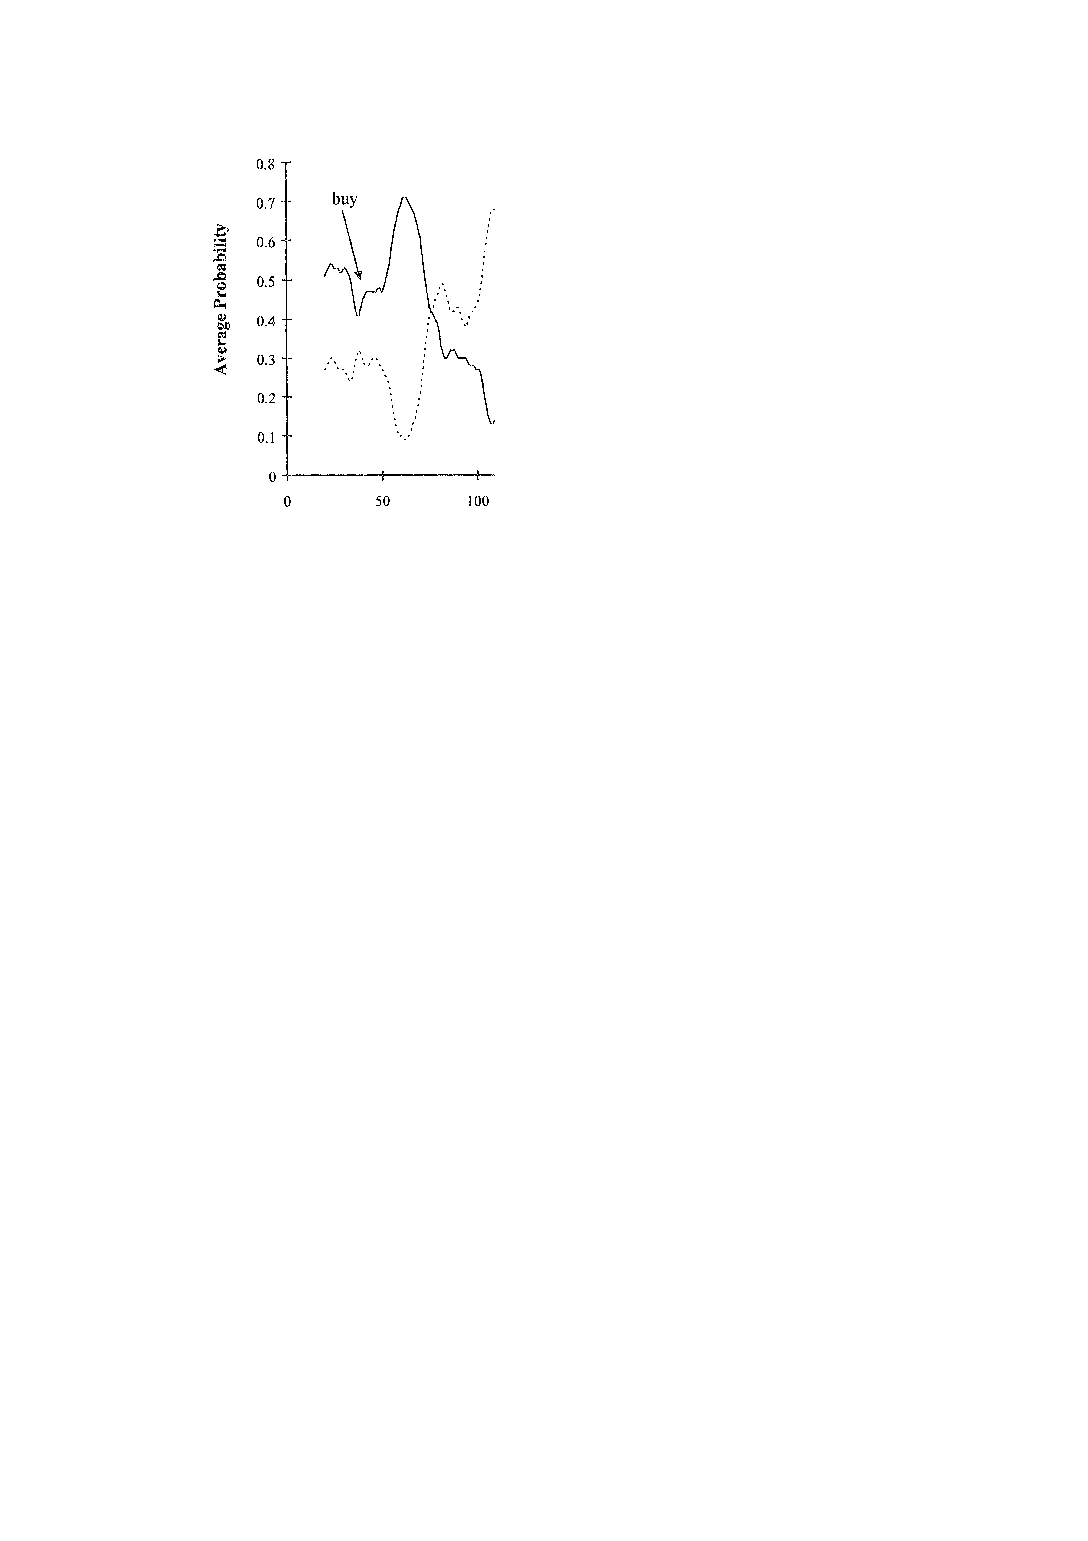
\includegraphics[width=0.17\paperwidth]{pics/Trade2} \hfill \hfill
	
	As the price goes up, the herd is broken: trading volume diminishes as rational traders drop out
\end{frame}


\begin{frame}{Herding with prices example (4)}
	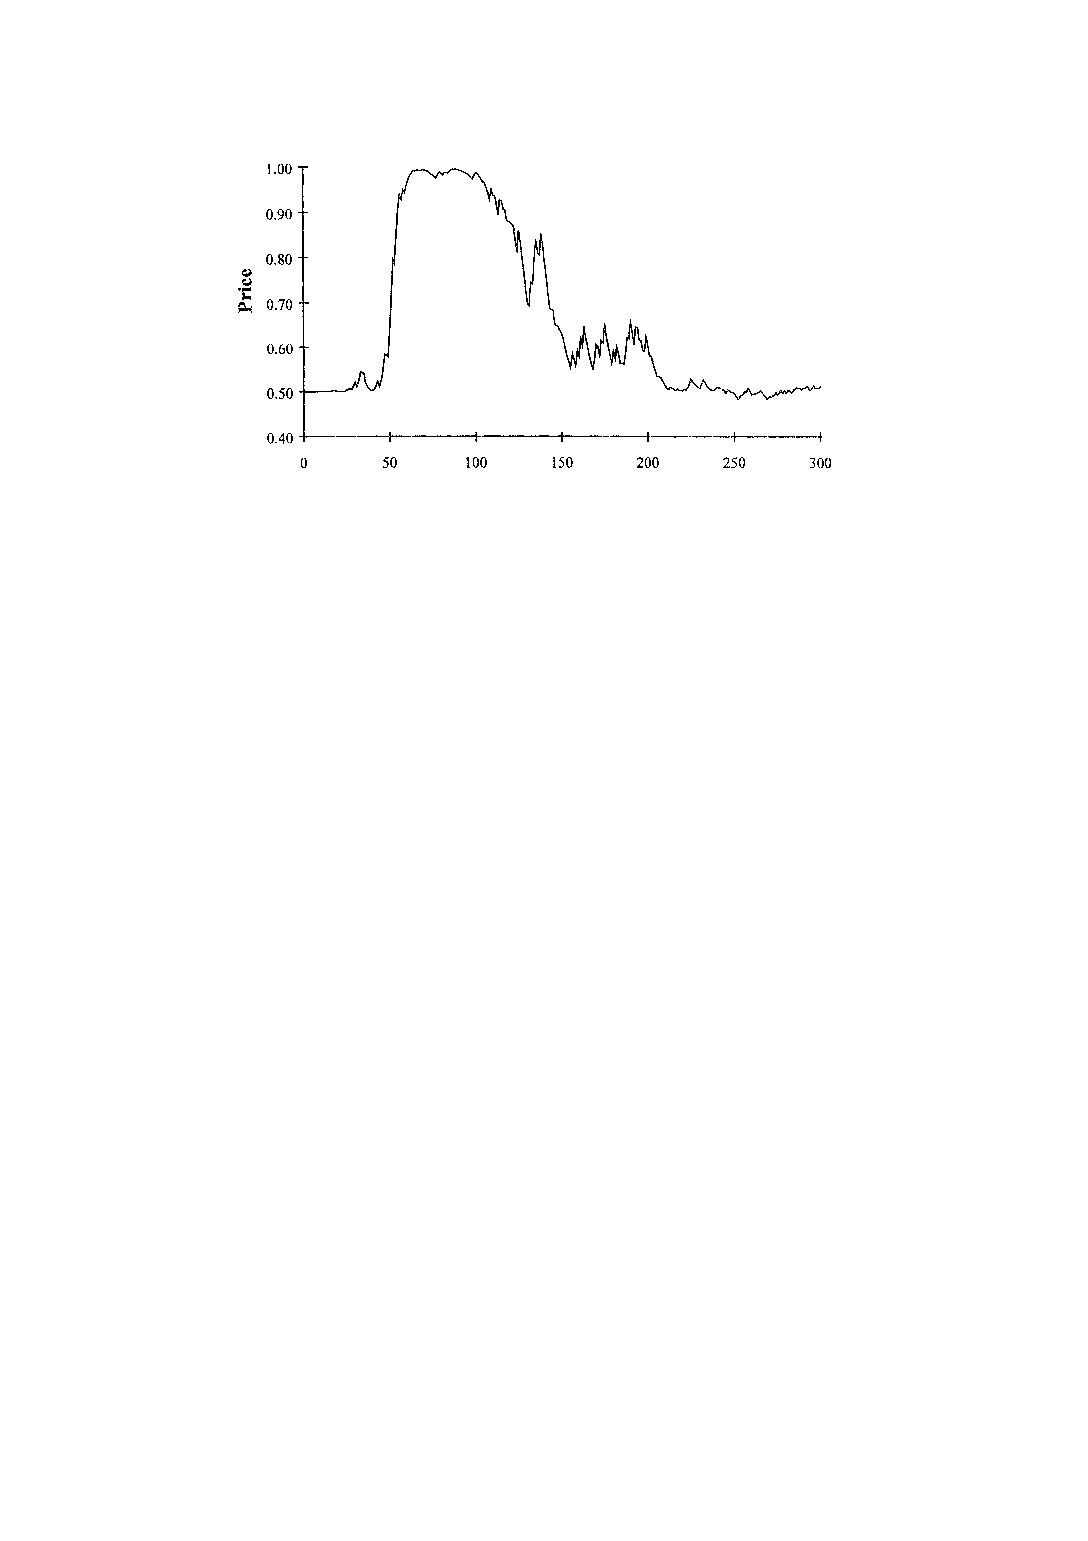
\includegraphics[width=0.4\paperwidth]{pics/PriceBubble}
	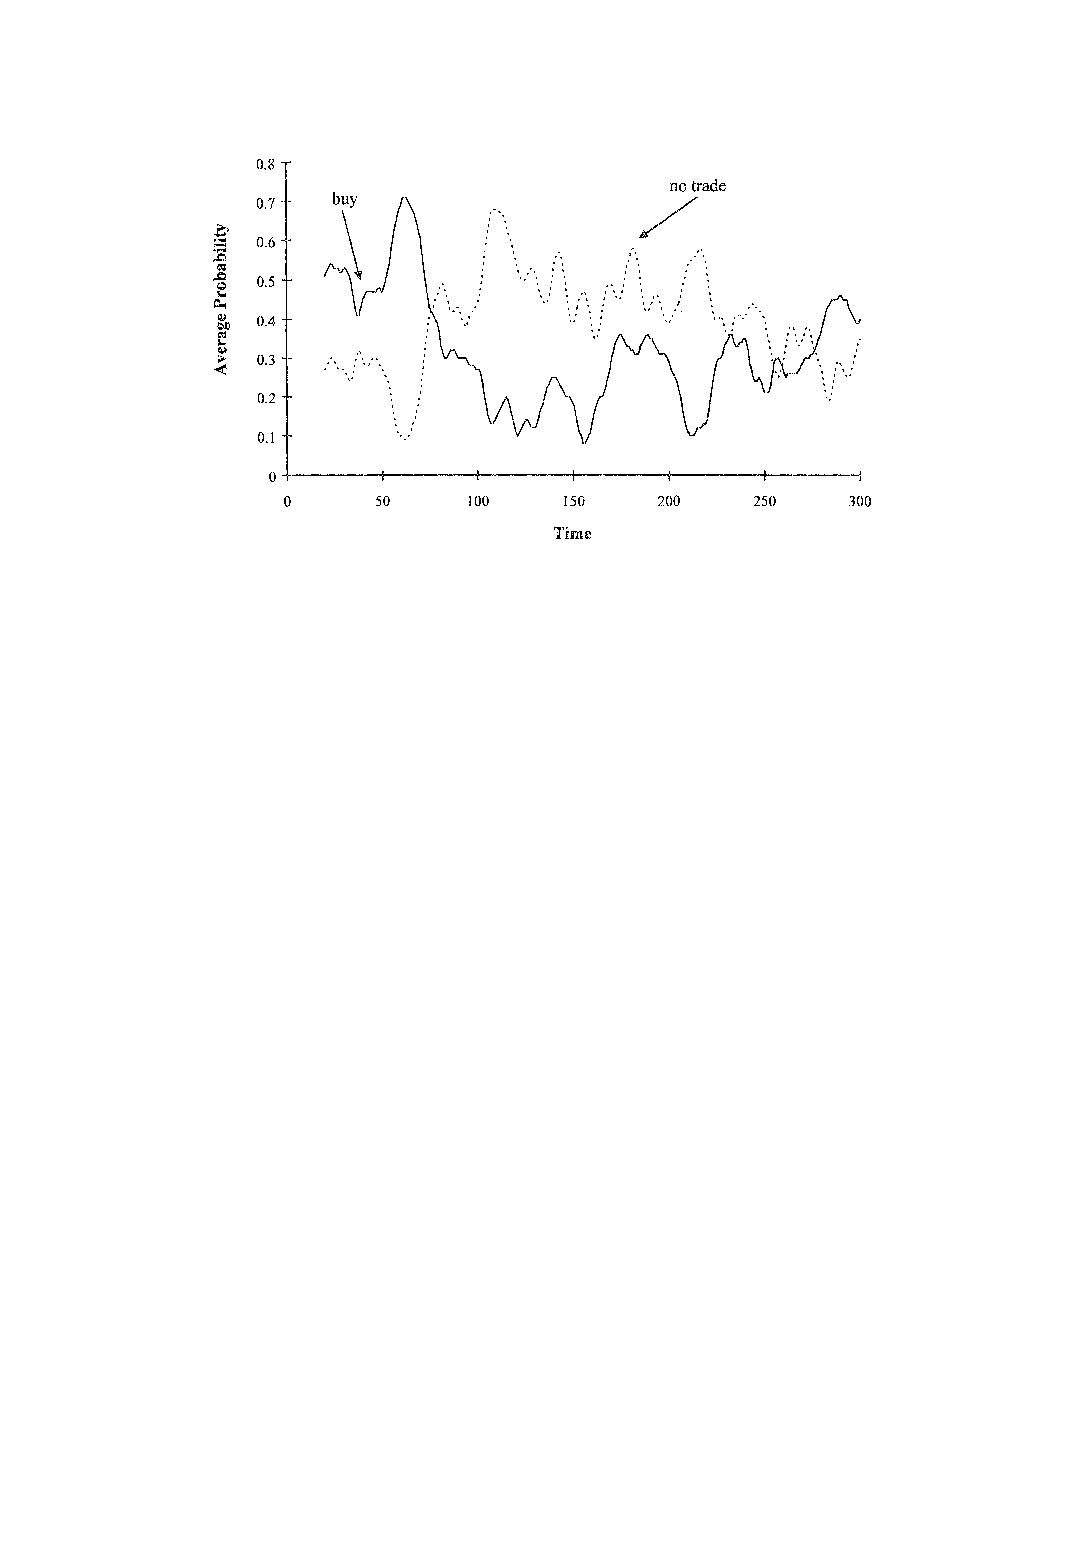
\includegraphics[width=0.4\paperwidth]{pics/TradeInBubble}
	
	As herd becomes apparent, MM realizes that only a few informative trades have been made $\rightarrow$ price toward 1/2
\end{frame}


\begin{frame}{Herding with prices example (5)}
	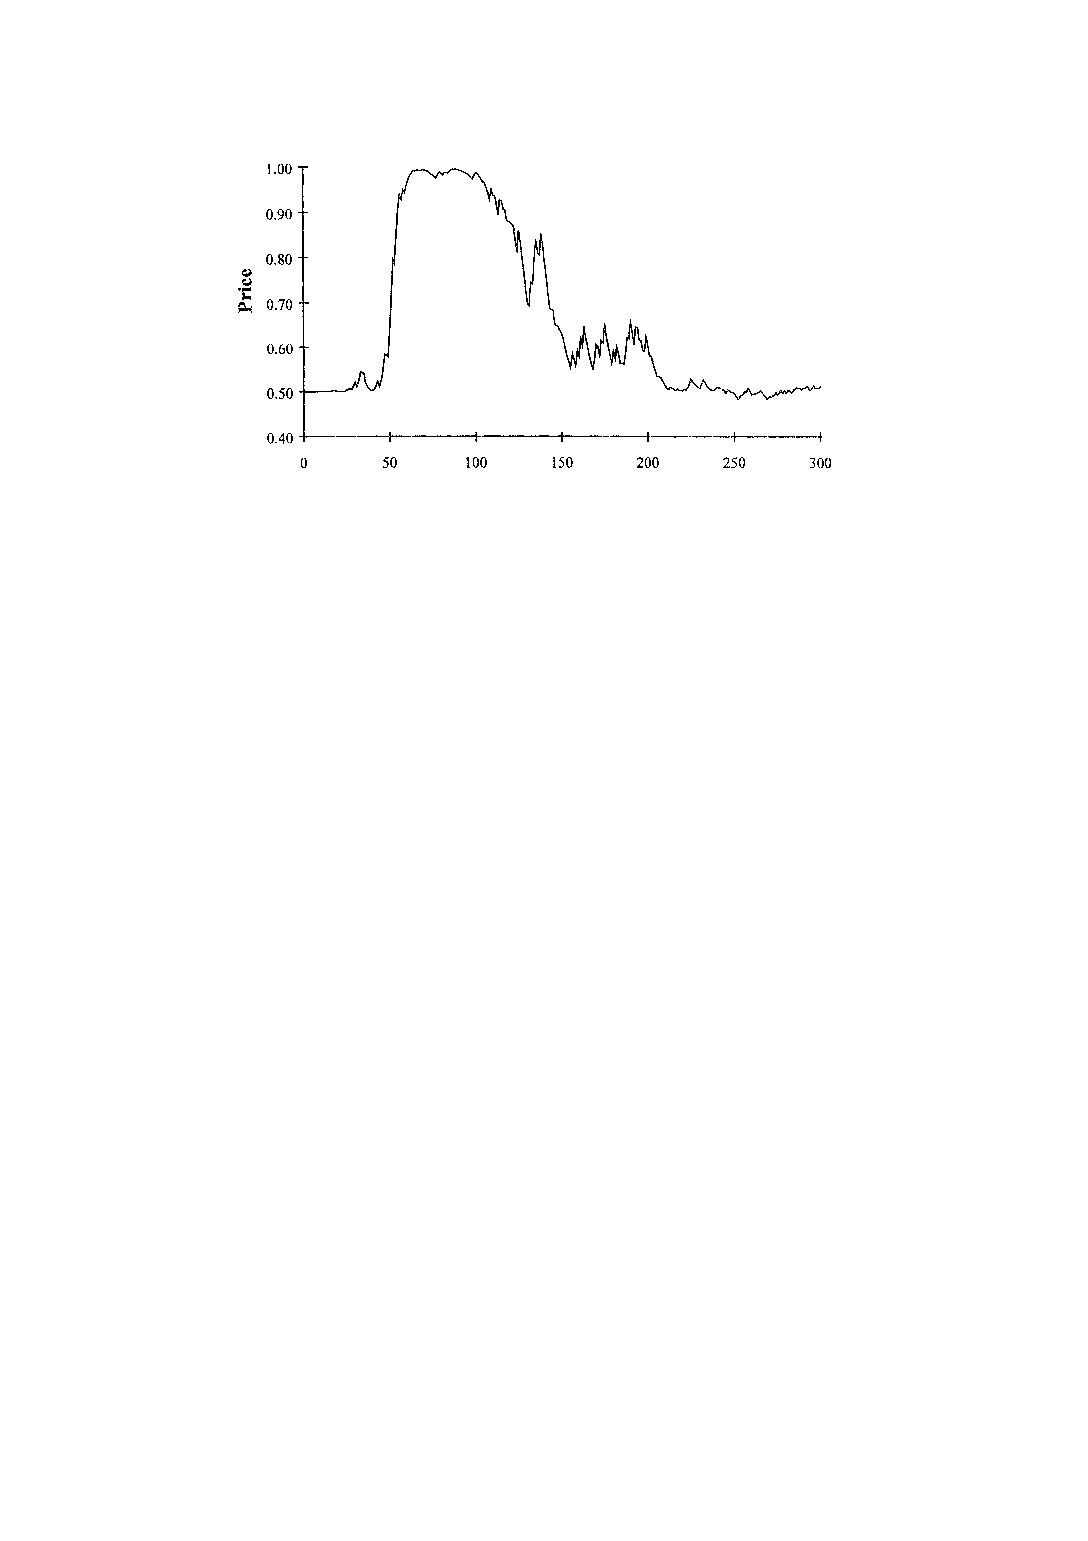
\includegraphics[width=0.4\paperwidth]{pics/PriceBubble}
	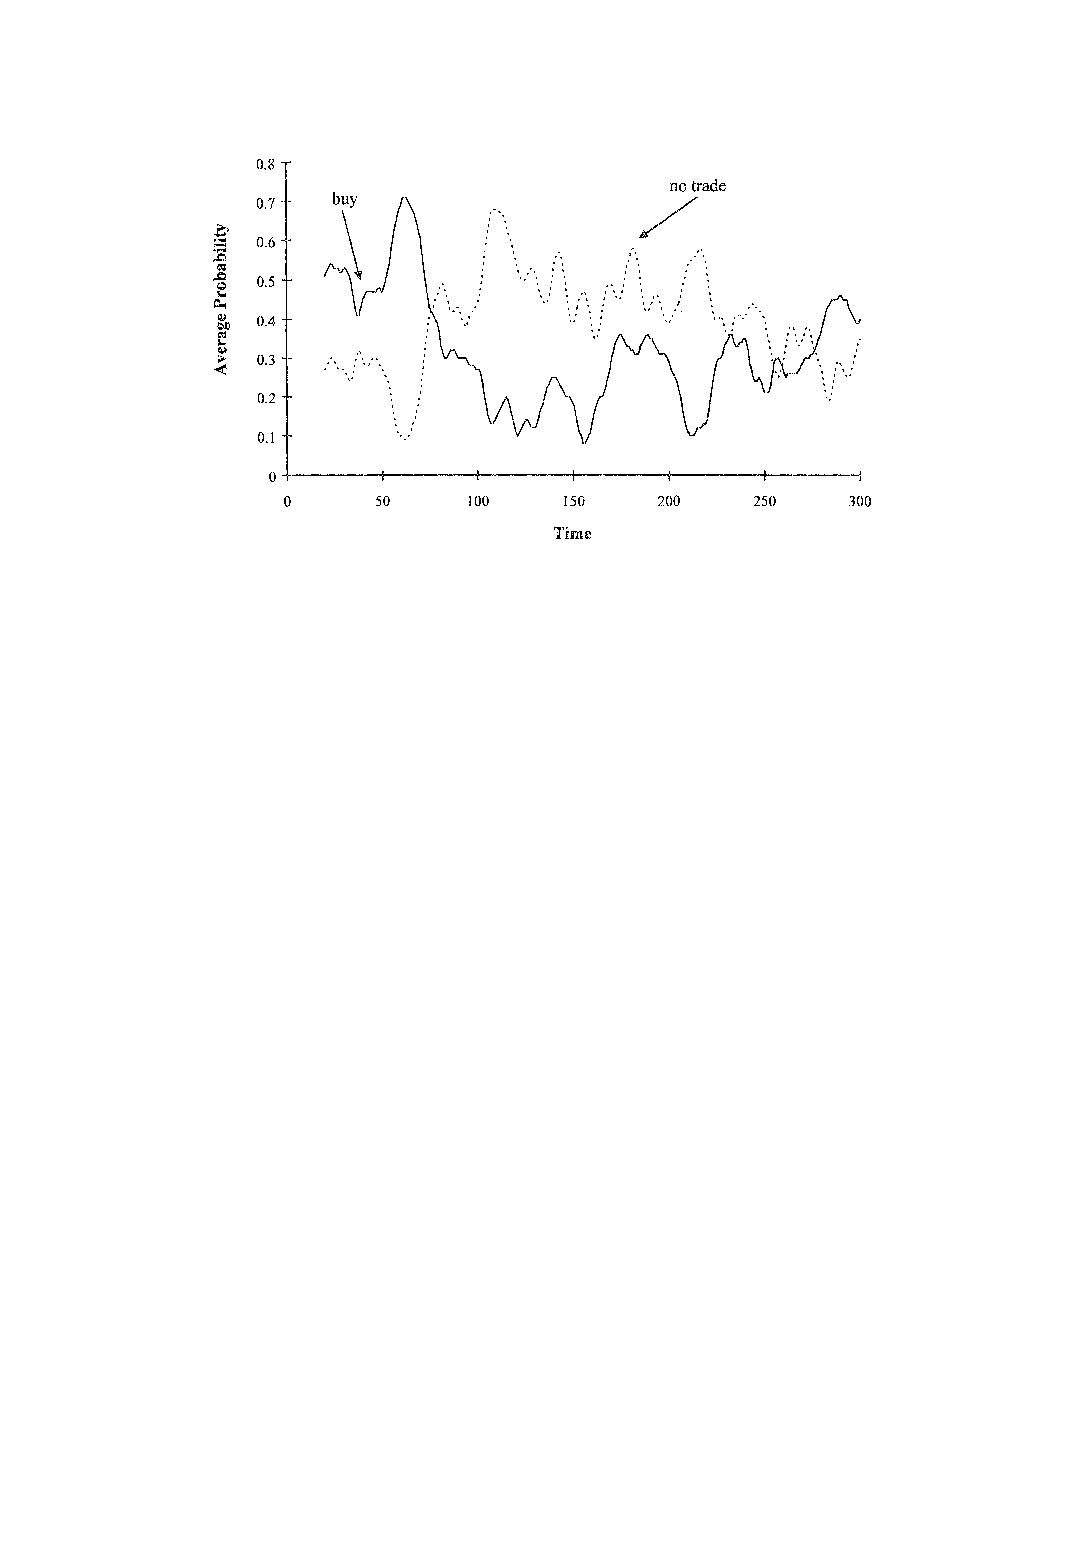
\includegraphics[width=0.4\paperwidth]{pics/TradeInBubble}
	
	Rational traders only re-enter in period 220: trade based on information (buy if high/sell if low)
	
	In the example, the price is persistently above the level that would ensue if traders pooled their information \hfill \hyperlink{az}{\beamerbutton{Back}}
\end{frame}


\end{document} 